\documentclass[notitlepage]{revtex4-1}

\usepackage{graphicx}
\usepackage{amsmath}
\usepackage[margin=5pt]{subfig}
\usepackage[usenames]{color}
% \usepackage{xspace}
\definecolor{darkgreen}{rgb}{0.00,0.50,0.25}
\definecolor{darkblue}{rgb}{0.00,0.00,0.67}
\newcommand{\figref}[1]{Fig.~\ref{#1}}
\usepackage[breaklinks,pdftitle={ZeroDB whitepaper}, pdfauthor={Michael Egorov},colorlinks,urlcolor=blue,citecolor=darkgreen,linkcolor=darkblue]{hyperref}
\usepackage[usenames]{color}
\graphicspath{{pdf/}}

\begin{document}

\title{ZeroDB whitepaper}

\author{M. Egorov}
\email{michael@zerodb.io}
\author{M. Wilkison}
\email{maclane@zerodb.io}

\begin{abstract}
ZeroDB is an end-to-end encrypted database that enables clients to operate on (search, sort, query, and share) encrypted data without exposing encryption keys or cleartext data to the database server.
The familiar client-server architecture remains, but query logic and encryption keys are pushed client-side.
Since the server has no insight into the nature of the data, the risk of a server-side data breach is eliminated.
Even if adversaries successfully infiltrate the server, they will not have access to the cleartext data.

ZeroDB provides end-to-end encryption while maintaining much of the functionality expected of a modern database, such as full-text search, sort, and range queries.
Additionally, ZeroDB uses proxy re-encryption and/or delta key technology to enable secure, granular sharing of encrypted data without exposing keys to the server and without sharing the same encryption key between all users of the database.
\end{abstract}

\date{\today}
\maketitle

\section{Introduction}

Review of existing systems needed:~\cite{cipherbase}~\cite{cryptdb}~\cite{gentry}~\cite{smart}

\section{Query protocol}

The basis of the end-to-end encrypted query protocol is as follows.
The client interacts with the server during the execution of a query over a series of round trips.
An encrypted index is stored on the server as a B-Tree, and the client traverses this index remotely to retrieve the necessary encrypted records.
The index consists of buckets which are encrypted before being uploaded to the server and only decrypted client-side.

\subsection{Equality query (using example of keyword search)}
\begin{figure}
	\begin{center}
        \subfloat[Encrypted index traversal example (simple keyword search)]{\label{fig:tree-traversal}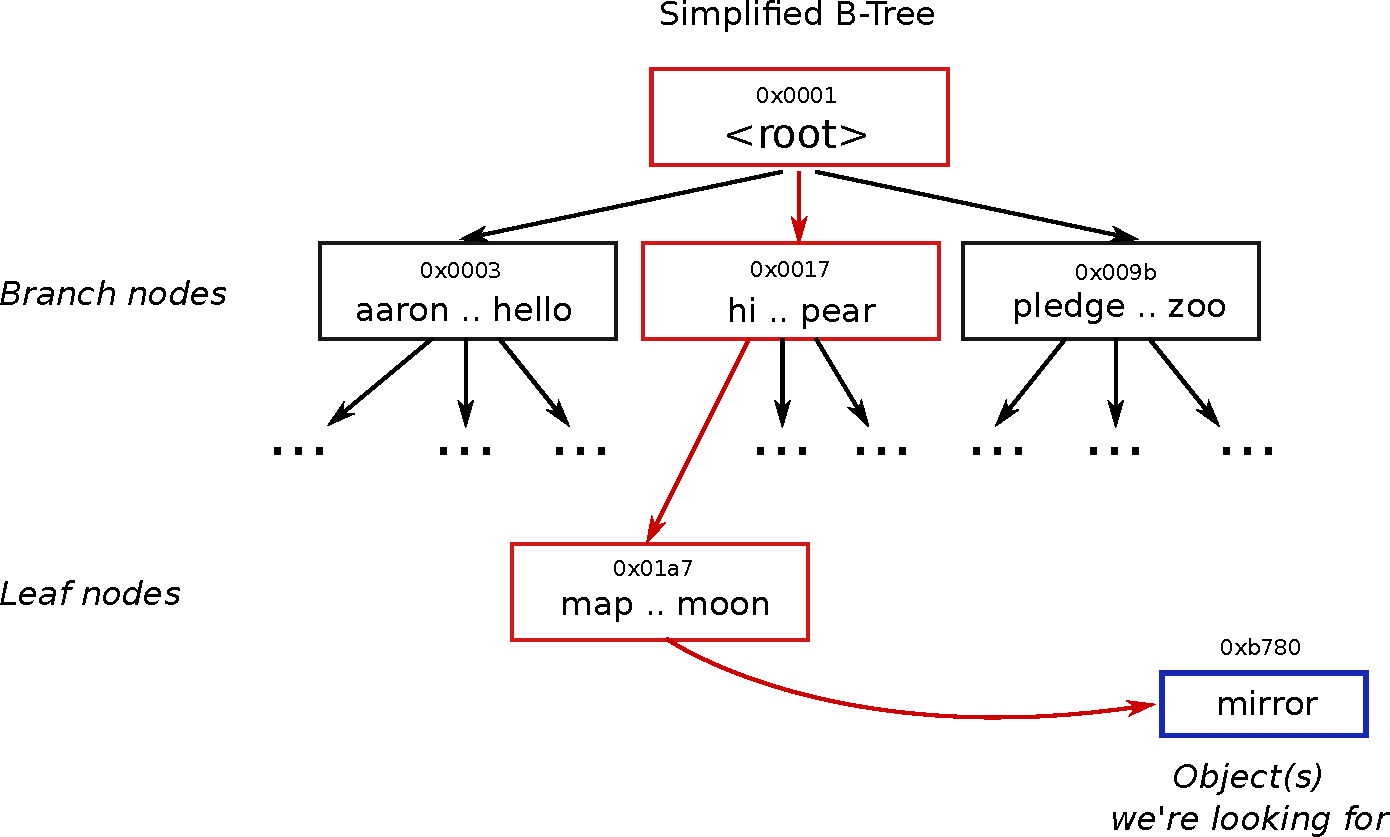
\includegraphics[width=0.47\columnwidth]{btree-traverse.pdf}}
        \qquad
        \subfloat[Sequence of client requests for traversal of the example index]{\label{fig:communication}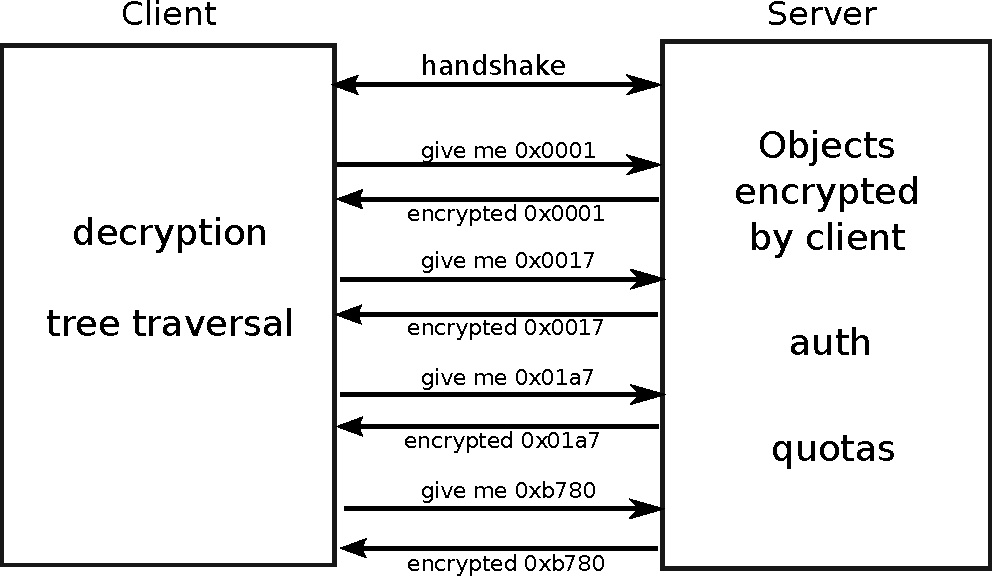
\includegraphics[width=0.47\columnwidth]{protocol.pdf}}
	\end{center}
    \caption{Search protocol for equality query using an example of keyword search}
	\label{fig:btree-protocol}
\end{figure}

In ZeroDB, indexes are structured as B-Trees~\figref{fig:tree-traversal}.
A B-Tree consists of buckets, each of which can be either a root, branch, or leaf node.
The leaf nodes of a tree point to the actual objects being stored.
Thus, searching the database is a simple tree traversal.

In order to make the database end-to-end encrypted yet still capable of performing queries, the client encrypts the buckets (at the time of creation or modification).
The server, which stores the buckets, never knows the encryption key used.
The objects referenced by the leaf nodes of the B-Tree indexes are also encrypted client-side.
As a result, the server does not know how individual objects are organized within the B-Tree or whether they even belong to an index at all.
Since ZeroDB is encryption agnostic, probabilistic encryption can be used so that the server cannot even compare objects for equality.

When a client performs a query, it asks the server to return buckets of the tree as it traverses the index remotely~\figref{fig:communication}.
Buckets can be cached client-side so that subsequent queries do not make unnecessary network calls.

The server is responsible for data replication, multi-version concurrency, object locking, user authentication, quotas, etc.
The client performs encryption/decryption and query logic.

\subsection{Range queries}

\begin{figure}
	\begin{center}
        \subfloat[Query searching for objects with a property $16 \le weight$, $limit=4$ (takes 4 requests w/o cache)]{\label{fig:range-query-iter}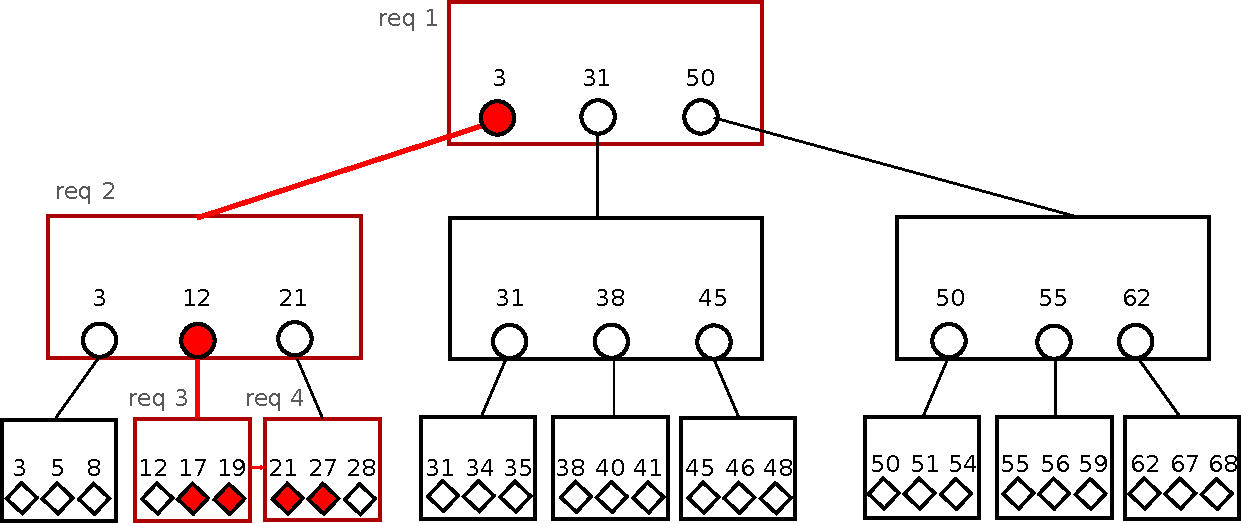
\includegraphics[width=0.47\columnwidth]{range-query-iter.pdf}}
        \qquad
        \subfloat[Query which fetches \emph{all} objects  with $16 \le weight \le 27$ (takes 3 requests w/o cache)]{\label{fig:range-query-star}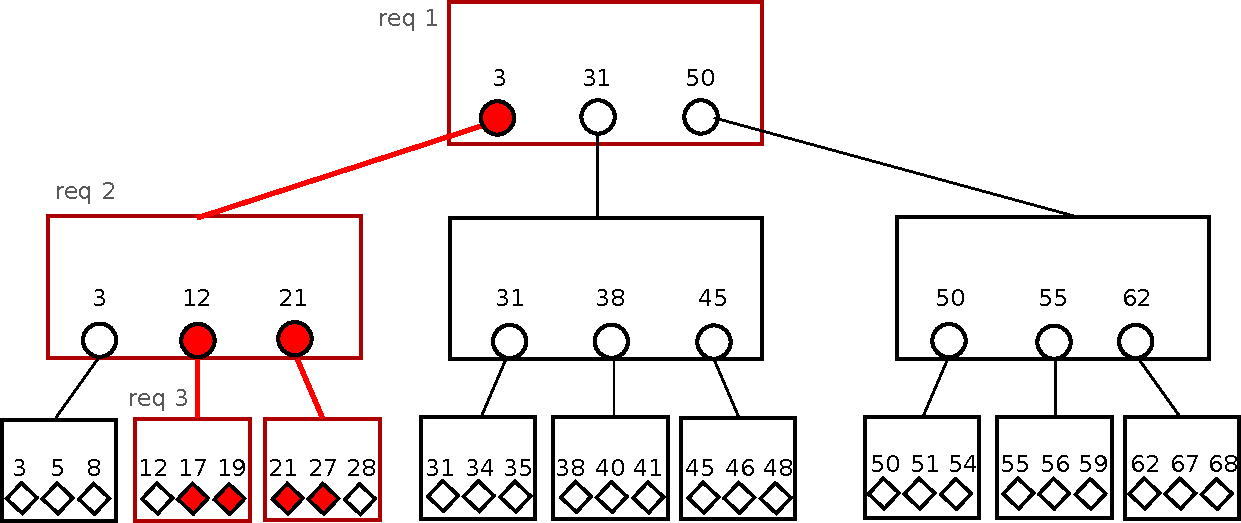
\includegraphics[width=0.47\columnwidth]{range-query-star.pdf}}
	\end{center}
	\caption{Range queries}
	\label{fig:range-query}
\end{figure}

When data are organized in B-Trees, doing range queries is easy.
Take an example having records \emph{Record} with an integer property \emph{weight}.
Data pointers to \emph{Record} objects are placed in a B-Tree sorted by \emph{weight}.

Two different types of range queries could be performed.
One is when we want a small subset of data in the beginning of the range (limit query).
In this case, we find a pointer to the beginning of the range~\figref{fig:range-query-iter}, then incrementally fetch subsequent buckets if the range occupies more than one, then bulk-fetch objects themselves by their pointers.

The other case is when we want to get \emph{all} objects in the range (select *).
We download subsection of B-Tree matching the range query level-by-level in logarithmic number of steps in this case~\figref{fig:range-query-star}.
To do that, we start with the root bucket.
Then, we download all the child buckets which match the range at once.
Then all children of those buckets, repeating until we get to the leaf nodes.
After that we (optionally) bulk-fetch all the objects which match the range query at once.
This is done in a way similar to prefetching all trees (Section~\ref{sec:bulk-fetching}).
Selecting all objects in a range reveals the approximate number of objects in this range to the server (the range and field names remain secret).

\subsection{Complex queries (multi-keyword search, multiple conditions)}

So far we described simple queries.
But queries may contain multiple conditions at the same time.
Depending on number of objects matching each condition and desired security properties we can use different approaches.
Making a query with ``or'' condition requires simply zip-joining two sorted datasets, so we do not consider that to be problematic.
Instead, let us consider a query where we select objects matching the condition $(v_1 = a) \,\&\, (v_2 = b)$ and ordered by $v_3$.

\subsubsection{Prefetch approach}
%    a) var1: BTree(var1 -> TreeSet(ids))
%       var2: BTree(var2 -> TreeSet(ids))
%       Take shorter treeset (say, for var1), fetch all ids
%       Traverse treeset for var2 in parallel to find all the ids from 1st treeset
%       Find order by traversing reverse index var3: BTree(id -> var3)
%
%       Example: any typical highly selective query
%       Pros: easy to reorder afterwards
%       Cons: very strong hint about how large the dataset is (unless reading more data than actually need), bad performance if words have ~same weights

In case the number of items with $v_1=a$ is small, it could be worthwhile to download the entire subset of object IDs matching this condition.
This could be practical in a multi-keyword search when one word is rare.

We can use the following indexes for this kind of query:
\begin{align*}
    & \mbox{BTree}(v_1 \rightarrow \mbox{TreeSet}(ids)),\\
    & \mbox{BTree}(v_2 \rightarrow \mbox{TreeSet}(ids)),\\
    & \mbox{BTree}(id \rightarrow v_3).
\end{align*}

First, we estimate which condition has the smallest number of matching elements.
We can do so by fetching ``contours'' of the B-Trees (corresponding to smallest and largest elements of the range respectively) in order to determine the height of the tree and approximate distance between the smallest and largest elements, knowing average size of a bucket, and it ``costs'' $H$ requests between client and server.

We prefetch a TreeSet for the most ``lightweight'' condition (Sec.~\ref{sec:bulk-fetching}).
Then we bulk-search~(Sec.~\ref{sec:parallel-traversal}) these IDs in the larger TreeSet (and if we do not find an ID in the leaf node, we drop it).

After that, we want to sort the small subset of fetched IDs by $v_3$.
We do a parallel traversal of the third B-Tree and find which value of $v_3$ corresponds to each ID.

This approach reveals the number of elements matching condition $v_1=a$ to the server, although the condition itself remains unknown.

\subsubsection{Preorder approach}

The prefetch approach could be slow and reveal too much information to the server.
So, whenever possible, values are pre-ordered in the index.
It works in the following way.

The composite index to make a query selecting objects matching the condition $(v_1 = a) \,\&\, (v_2 = b)$ and ordered by $v_3$ is:
\begin{equation*}
    \mbox{BTree}((v_1, v_2) \rightarrow \mbox{BTree}(v_3 \rightarrow \mbox{TreeSet}(ids))).
\end{equation*}
For this query, we find a B-Tree (or multiple B-Trees) corresponding to the conditions and lazily traverse them in order of $v_3$.
This makes limit orders much more performant and does not leak information about possible dataset size to the server.

\subsubsection{Doing set intersection server-side}

\begin{figure}
	\begin{center}
        \subfloat[Branch node]{\label{fig:keytree-branch-node}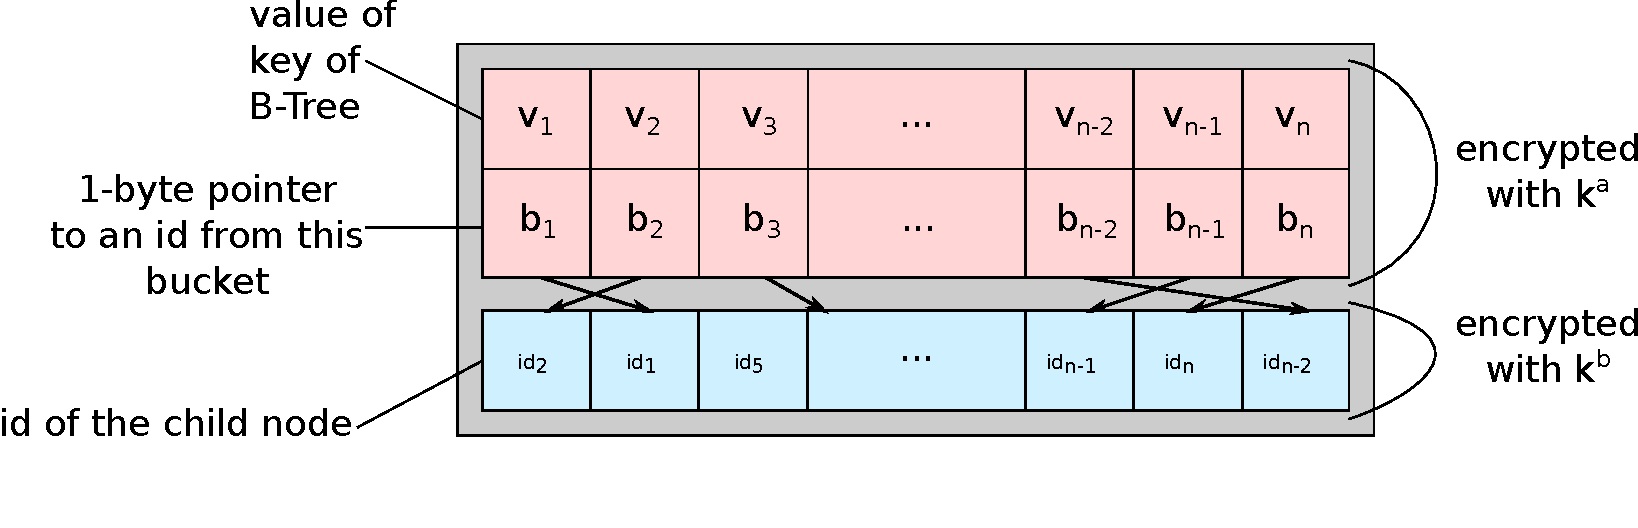
\includegraphics[width=0.47\columnwidth]{keytree-branch-bucket.pdf}}
        \qquad
        \subfloat[Leaf node]{\label{fig:keytree-leaf-node}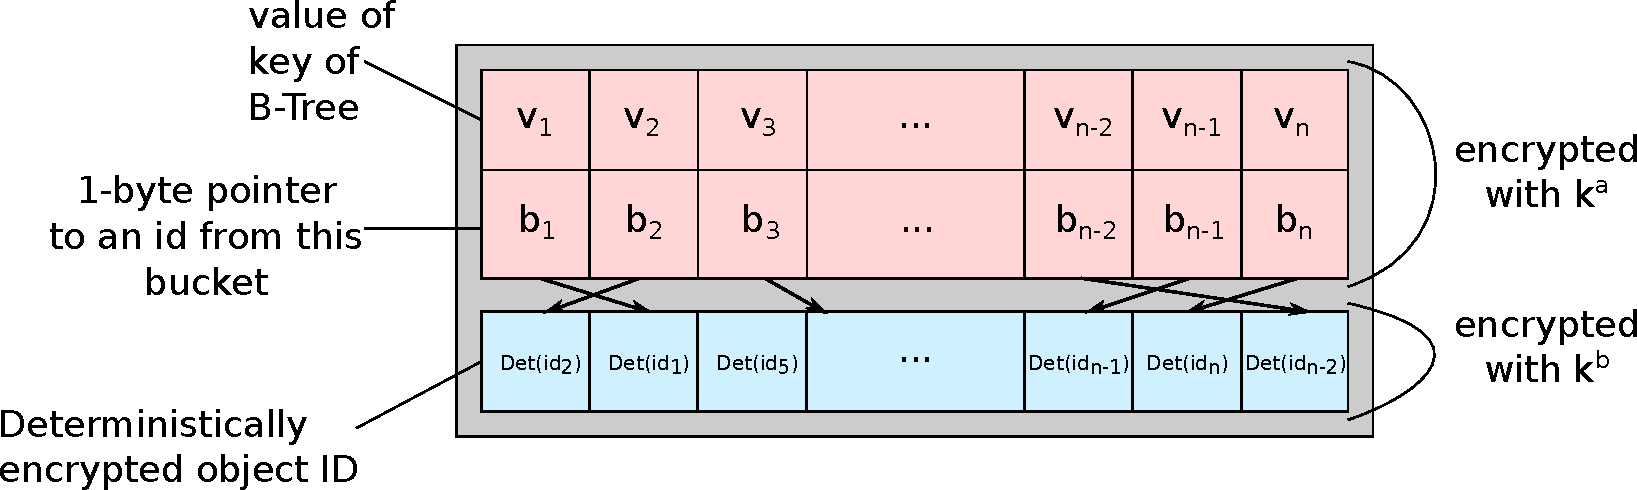
\includegraphics[width=0.47\columnwidth]{keytree-leaf-bucket.pdf}}\\
        \subfloat[Tree of keys]{\label{fig:keytree}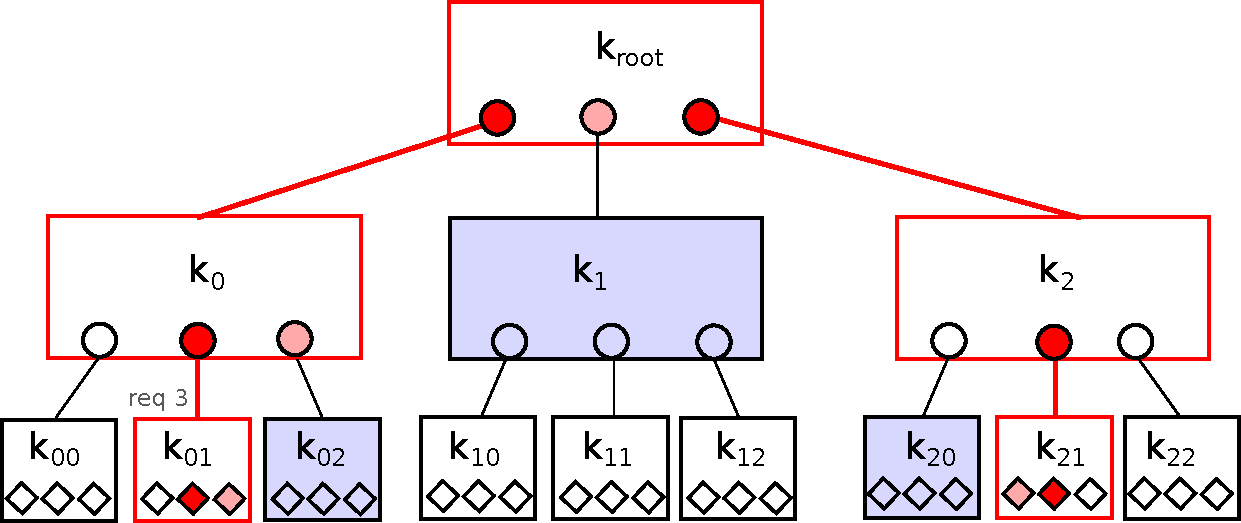
\includegraphics[width=0.7\columnwidth]{keytree.pdf}}
	\end{center}
    \caption{B-Tree structure which supports server-side set operations.
    TBC\ldots}
	\label{fig:server-side-sets}
\end{figure}
%   c)  Less secure: opening deterministically encrypted ids to the server
%       and let it do the interesection of result sets.
%       // picture from notes to show what it is

%       All the considerations above are also valid for joins

%       ** All "btrees of treesets" or "btrees(var1) of btrees(var2)" can be
%       replaced with indexes on tuples (var1, var2) to have the same total
%       index height for all values of var2 (which could have performance and
%       security benefits)

%   "Proper" joins are a little unclear. We don't want to open deterministically encrypted *values* to the server
%   b/c it opens up too much information for statistical analysis.
%   We can use default ZODB approach of events/subscribers when related objects are modified instead

\subsection{Optimizations specific for remote client}

In most cases, all the query logic in ZeroDB happens client-side, e.g. client and storage are separated by a network channel with high latency.
Therefore, we use two primitives specific for this architecture.

\begin{figure}
	\begin{center}
        \subfloat[When a tree (or sub-tree) is small, it can be fully pre-fetched to the client]{\label{fig:fetch-tree}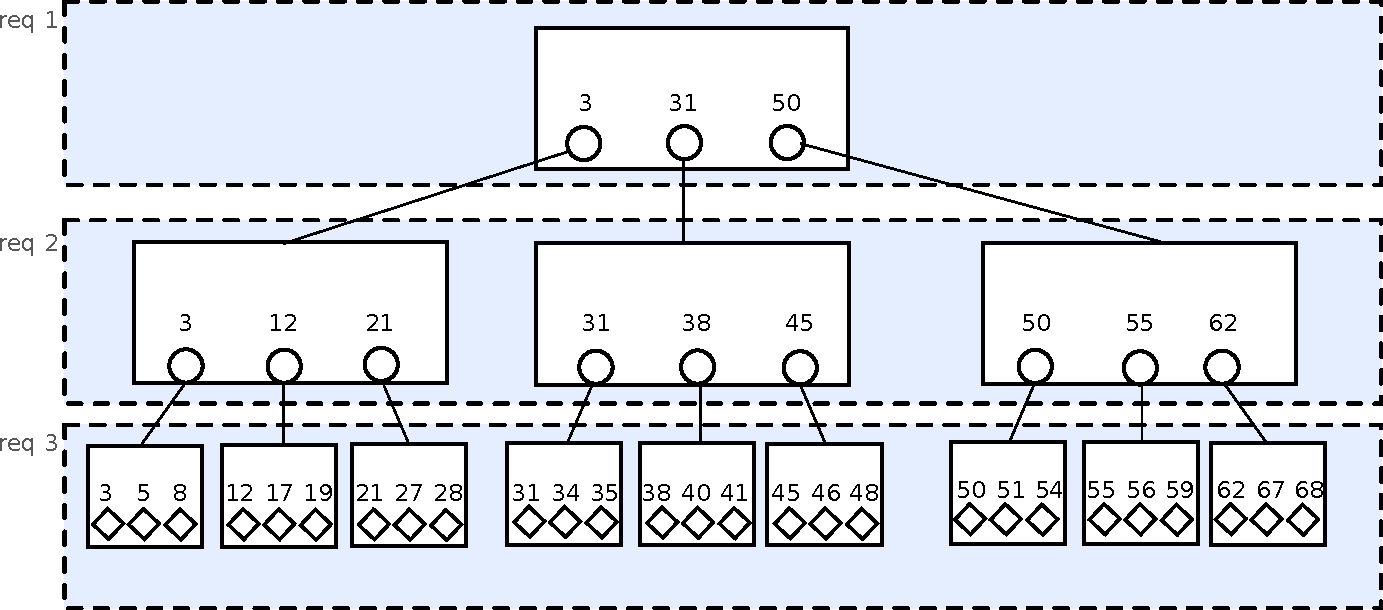
\includegraphics[width=0.47\columnwidth]{fetch-tree.pdf}}
        \qquad
        \subfloat[When multiple branches of the tree needs reading/updating, tree traversal can be done in parallel]{\label{fig:parallel-traversal}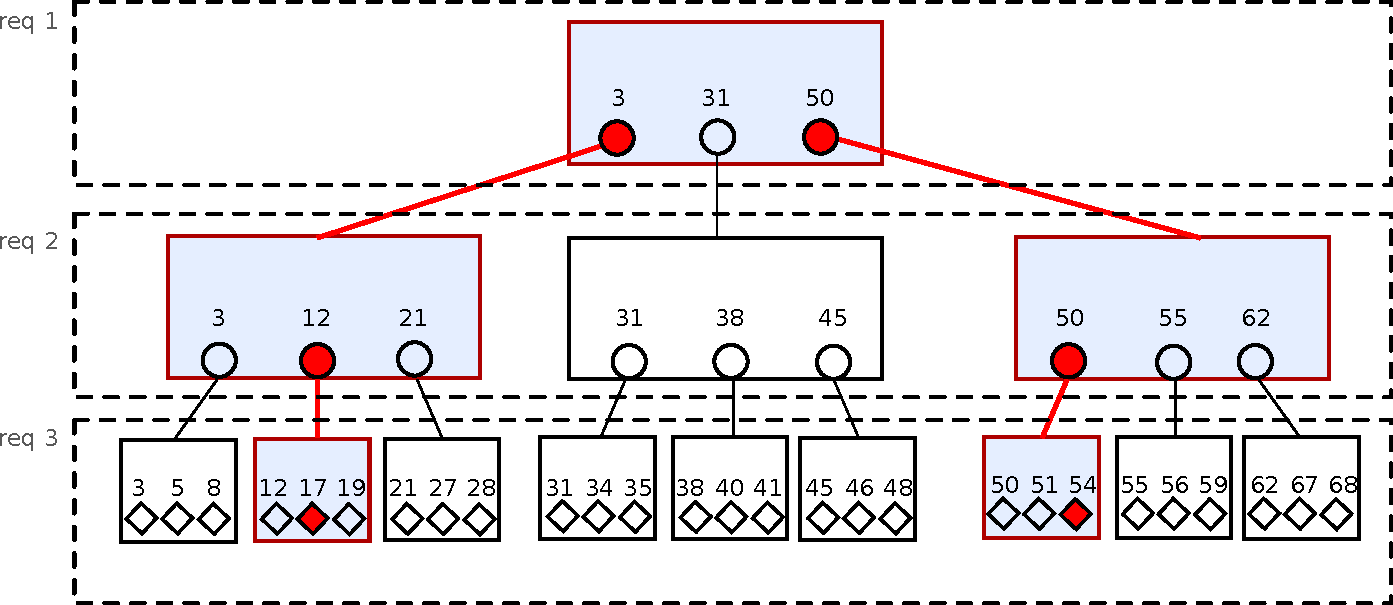
\includegraphics[width=0.47\columnwidth]{parallel-traversal.pdf}}
	\end{center}
    \caption{ZeroDB-specific optimizations of working with B-Trees. Allows to pre-fetch a tree or find multiple values in number of steps equal to the tree height}
	\label{fig:tree-traversal-optimizations}
\end{figure}

\subsubsection{Bulk-fetching small (sub)trees}
\label{sec:bulk-fetching}

When a tree (or sub-tree) is small enough, it could be more performant to fetch the entire tree to the client.
We do not need to do that bucket-by-bucket, as one would do with an index stored on a local hard drive, but in a logarithmic number of steps.

In order to do that, we fetch the root first~\figref{fig:fetch-tree}.
The client unpacks the root bucket and fetches all its children in one query.
Then it unpacks all the child nodes and learns the IDs of their children.
This process continues until the entire B-Tree is fetched.
Thus, the number of queries is equal to the height of the B-Tree, $H$, proportional to the logarithm of its size, $\log{S_{\mbox{ix}}}$.

When we fetch a tree, we implicitly show the number of objects it contains, $S_{\mbox{ix}}$, to the server.
Based on the size of the read data, the observer would be able to infer a number close to $S_{\mbox{ix}}$ and associate it with the bucket IDs just read.
Therefore, this technique should be used as rarely as possible, combined with reading other data at the same time or with oblivious RAMs~\cite{path-oram,burst-oram,oram-multicloud,ods-wang-2014}.
The latter would prevent the observer from learning bucket IDs.

\subsubsection{Parallel tree traversal}
\label{sec:parallel-traversal}

Often queries involve several values of the same field (or different fields).
For example, indexing a new document containing $100$ words could be an expensive operation since it would involve $100\,H$ requests to the server, making the performance defined by client-server latency very poor.

In order to fix that, we traverse the B-Tree in parallel~\figref{fig:parallel-traversal}.
We first fetch the root of the tree.
Then, we fetch only those child-buckets of the root which are relevant to the values in our query.
Then, we fetch only the relevant children of those, etc.
This way, we do tree traversal for all the necessary values in $H$ steps.

When we do parallel traversal, the server would be able to see access patterns but it would not be able to distinguish access patterns belonging to each of the values individually.

\section{Sharing data}

\section{Security analysis}

\section{Performance}

\subsection{Unfolding trees with subtrees into one tree}

\subsection{Benchmarks}

\bibliography{zerodb}

\end{document}

